\documentclass[border=3pt,tikz]{standalone}
\usetikzlibrary{positioning}
\begin{document}
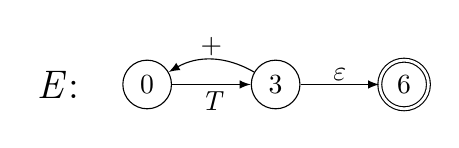
\begin{tikzpicture}
  % E
  \node (E) at (0,0) {\Large \textit{E}:};
  \node[circle,draw=black,right=1.21em of E] (zero) {0};
  \node[circle,draw=black,right=of zero] (three) {3};
  \node[circle,double,double distance=1pt,draw=black,right=of three] (six) {6};

  \path[-latex,draw]
  (zero) edge node[below=-1pt]{\(\textit{T}\)} (three)
  (three) edge node[above=-2pt]{\(\varepsilon\)} (six)
  (three) edge[out=150,in=30,distance=1.2em] node[above=-2pt]{\(+\)} (zero);
\end{tikzpicture}
\end{document}
